\documentclass{article}
\usepackage{amsmath}
\usepackage{mathtools}
\usepackage{gensymb}
\usepackage[a4paper,inner=1.5cm,outer=1.5cm,top=2cm,bottom=0.5cm]{geometry} 
\usepackage{xcolor}                    
\usepackage{tikz}                           
\usepackage{multicol}
\usepackage{pgfplots}
\usetikzlibrary{calc}
\usetikzlibrary{intersections}
\usetikzlibrary{intersections,calc,angles,quotes}
\usetikzlibrary{shapes,arrows,positioning,decorations.pathreplacing,calc}
\usetikzlibrary{calc,angles,positioning,intersections,quotes,decorations.markings}
\usepackage{tkz-euclide}
\usetikzlibrary{backgrounds}
\usetikzlibrary{calc,through}
\usetikzlibrary{angles}
\usetikzlibrary{fadings}
\usetikzlibrary{shapes.geometric}
\usetikzlibrary{shapes.symbols}
\usepackage{draftwatermark}
\usepackage{mathptmx}

\SetWatermarkText{\textcolor{black!30}{Mathema Shukur}}
\SetWatermarkFontSize{2 cm}
\usepackage[utf8]{inputenc}
\usepackage{fontspec}

\setmainfont{[Kalpurush.ttf]}
\newfontface{\en}{[Arial.ttf]} %%this is optional, if you want to use a secondary font. Any english font is supported
\newlength\Radius
\setlength\Radius{4cm}
\begin{document} 
	\Large
	\textcolor{red}{Welcome To} 
	\\
	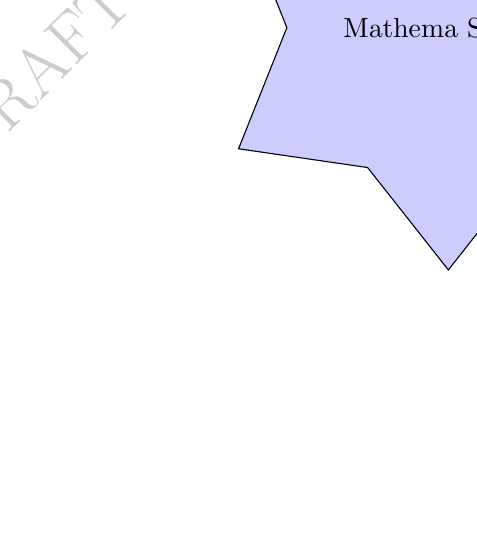
\begin{tikzpicture}
		\tikz \node [fill=blue!20,star,star points=6,draw] {Mathema Shukur };
	\end{tikzpicture}
	\\
	যাদের জন্যে প্রযোজ্যঃ  	\textcolor{magenta}{একাদশ ও দ্বাদশ শ্রেণীর শিক্ষার্থী} \\
	বিষয়ঃ \textcolor{magenta}{উচ্চতর গণিত ১ম পত্র} \\
	অধ্যায়ঃ \textcolor{magenta}{৩-সরলরেখা}\\ 
	Subtopicঃ  \textcolor{magenta}{ অভিন্ন  সরলরেখার শর্ত  কী?  Identical Straight Lines   }\\
\\
\textcolor{blue}{	দুইটি সাধারণ সমীকরণ একই সরলরেখা নির্দেশ করার শর্ত }\\
		$a_1x+b_1y+c_1=0$ এবং	$a_2x+b_2y+c_2=0$  একই সরলরেখা নির্দেশ করলে $\frac{a_1}{a_2}=\frac{b_1}{b_2}=\frac{c_1}{c_2}$\\ 
		\\ 
	যশোর বোর্ড-২০২১\\ 
$2x+3y=7$ এবং $3px-5qy+15=0$ সমীকরণ দুইটি একই সরলরেখা প্রকাশ করলে ধ্রুবক $p$ এবং $q$ এর মান কত? \\
\begin{multicols}{2}
	\begin{align*}
		2x+3y&=7\\
		\\
		2x+3y-7&=0\\
		\\
		a_1=2,\quad b_1&=3,\quad c_1=-7
	\end{align*}
	\\
	\begin{align*}
		3px-5qy+15&=0\\
		\\
		a_2=3p,\quad b_2&=-5q,\quad c_2=15\\
	\end{align*}
\end{multicols}
\begin{align*}
	\frac{a_1}{a_2}=\frac{b_1}{b_2}&=\frac{c_1}{c_2}\\
	\\
	\frac{2}{3p}=\frac{3}{-5q}&=\frac{-7}{15}
\end{align*}
\begin{multicols}{2}
\begin{align*}
	\frac{2}{3p}&=\frac{-7}{15}\\
	\\
	-21p&=30\\
	\\
	p&=-\frac{30}{21}\\
	\\
	p&=-\frac{10}{7}
\end{align*}
\\
\begin{align*}
	\frac{3}{-5q}&=\frac{-7}{15}\\
	\\
	35q&=45\\
	\\
	q&=\frac{45}{35}\\
	\\
	q&=\frac{9}{7}
\end{align*}	
\end{multicols}
দিনাজপুর বোর্ড-২০১৩\\
$ax+by=c$ এবং $x\,\,\cos \alpha+ y\,\,\sin \alpha=p$ একই সরলরেখা নির্দেশ করলে দেখাও যে , $p=\pm \frac{c}{\sqrt{a^2+b^2}}$\\ 
\begin{multicols}{2}
	\begin{align*}
	ax+by&=c\\
	\\
	ax+by-c&=0\\
	\\
	a_1=a,\quad b_1=b,\quad c_1=-c
\end{align*}
\\
\begin{align*}
	x\,\,\cos \alpha+ y\,\,\sin \alpha&=p\\
	\\
	x\,\,\cos \alpha+ y\,\,\sin \alpha-p&=0\\
	\\
	a_2=\cos \alpha,\quad b_2&=\sin \alpha,\quad c_2=-p
\end{align*}
\end{multicols}
\begin{align*}
	\frac{a_1}{a_2}=\frac{b_1}{b_2}&=\frac{c_1}{c_2}\\
	\\
	\frac{a}{\cos \alpha}=\frac{b}{\sin \alpha}&=\frac{-c}{-p}
\end{align*}
\begin{multicols}{2}
\begin{align*}
	\frac{a}{\cos \alpha}&=\frac{c}{p}\\
	\\
	c\,\,\,	\cos \alpha&= a\,\,p\\
	\\
	\cos \alpha &=\frac{a\,\,p}{c}
\end{align*}
\\
\begin{align*}
	\frac{b}{\sin \alpha}&=\frac{c}{p}\\
	\\
	c\,\,\sin \alpha &=b\,\,p\\
	\\
	\sin \alpha &=\frac{b\,\,p}{c}
\end{align*}
\end{multicols}
\begin{align*}
	\sin^2 \alpha+\cos^2 \alpha &=1\\
	\\
	\left(\frac{b\,\,p}{c}\right)^2+\left(\frac{a\,\,p}{c}\right)^2&=1\\
	\\
	\frac{b^2\,\,p^2}{c^2}+\frac{a^2\,\,p^2}{c^2}&=1\\
	\\
	b^2\,\,p^2+a^2\,\,p^2&=c^2\\
	\\
	p^2(a^2+b^2)&=c^2\\
	\\
	p^2&=\frac{c^2}{a^2+b^2}\\
	\\
	p&=\pm \sqrt{\frac{c^2}{a^2+b^2}}\\
	\\
	p&=\pm \frac{c}{\sqrt{a^2+b^2}}
\end{align*}
	(BUET-2005-2006) \\
	$k$ এর কোন মানের জন্য  $x-y=3$,\qquad $2x-2y=k$ সমীকরণজোটের অসংখ্য সমাধান থাকবে ?\\
	\begin{multicols}{2}
	\begin{align*}
		x-y&=3\\
		\\
		x-y-3&=0\\
		\\
		a_1=1,\quad b_1&=-1,\quad c_1=-3\\
	\end{align*}
	\\
	\begin{align*}
		2x-2y&=k\\
		\\
		2x-2y-k&=0\\
		\\
		a_2=2,\quad b_2&=-2,\quad c_2=-k
	\end{align*}
	\end{multicols}
\begin{align*}
	\frac{a_1}{a_2}=\frac{b_1}{b_2}&=\frac{c_1}{c_2}\\
	\\
	\frac{1}{2}=\frac{-1}{-2}&=\frac{-3}{-k}\\
	\\
	\frac{1}{2}&=\frac{3}{k}\\
	\\
	k&=6
\end{align*}
\\
	রাজশাহী বিশ্ববিদ্যালয় ভর্তি পরীক্ষা ২০১৯-২০২০\\
	$3x+\sqrt{3}y+2=0$ এবং $x\,\,\cos \alpha+ y\,\,\sin \alpha=p$ একই সরলরেখা নির্দেশ করলে $\alpha$ এবং  $p$ এর মান নির্ণয় কর ।\\  
	\begin{multicols}{2}
		\begin{align*}
		3x+\sqrt{3}y+2&=0\\
		\\
		a_1=3,\quad b_1=\sqrt{3},\quad c_1=2
	\end{align*}
	\\
	\begin{align*}
		x\,\,\cos \alpha+ y\,\,\sin \alpha&=p\\
		\\
		x\,\,\cos \alpha+ y\,\,\sin \alpha-p&=0\\
		\\
		a_2=\cos \alpha,\quad b_2&=\sin \alpha,\quad c_2=-p
	\end{align*}
	\end{multicols}
\begin{align*}
	\frac{a_1}{a_2}=\frac{b_1}{b_2}&=\frac{c_1}{c_2}\\
	\\
	\frac{3}{\cos \alpha}=\frac{\sqrt{3}}{\sin \alpha}&=\frac{2}{-p}\\
\end{align*}
\begin{multicols}{2}
\begin{align*}
	\frac{3}{\cos \alpha}&=\frac{2}{-p}\\
	\\
	2\,\,\cos \alpha&=-3\,p\\
	\\
	\cos \alpha&=\frac{-3\,\,p}{2}
\end{align*}
\\
\begin{align*}
	\frac{\sqrt{3}}{\sin \alpha}&=\frac{2}{-p}\\
	\\
	2\,\,\sin \alpha&=-\sqrt{3}\,\,p\\
	\\
	\sin \alpha&=\frac{-\sqrt{3}\,\,p}{2}
\end{align*}
\end{multicols}
\begin{multicols}{2}
\begin{align*}
	\sin^2 \alpha+\cos^2\alpha&=1\\
	\\
	\left(\frac{-\sqrt{3}\,\,p}{2}\right)^2+\left(\frac{-3\,\,p}{2}\right)^2&=1\\
	\\
	\frac{3\,p^2}{4}+\frac{9\,\,p^2}{4}&=1\\
	\\
	3\,p^2+9\,p^2&=4\\
	\\
	12\,\,p^2&=4\\
	\\
	p^2&=\frac{4}{12}\\
	\\
	p^2&=\frac{1}{3}\\
	\\
	p&= \frac{1}{\sqrt{3}}
\end{align*}
\\
\begin{align*}
	\frac{\sin \alpha}{\cos \alpha}&=\frac{\frac{-\sqrt{3}\,\,p}{2}}{\frac{-3\,\,p}{2}}\\
	\\
	\tan \alpha&=\frac{\sqrt{3}}{3}\\
	\\
	\tan \alpha&=\frac{1}{\sqrt{3}}\\
	\\
	\alpha&=30\degree \\
\end{align*}
\\

যেহেতু $\sin \alpha$ এবং  $\cos \alpha$ এর মান ঋণাত্মক \\
\\
সুতরাং $\alpha=180\degree+30\degree=210\degree$\\
\end{multicols}

\end{document}